\documentclass[12pt]{article}

\usepackage[a4paper,margin=1in]{geometry}

\usepackage{natbib}
\usepackage{amsmath,amssymb,amsfonts}
\usepackage{algorithmic}
\usepackage{graphicx}
\usepackage{textcomp}
\usepackage{xcolor}
\usepackage{tabularx}
\usepackage{booktabs}   % add in preamble
\usepackage{ragged2e}
\usepackage{titlesec}
\usepackage{subcaption}
\usepackage{pgfplots}
\pgfplotsset{compat=1.18}

% float flexibility to avoid figure-only pages where possible
\renewcommand{\topfraction}{0.9}
\renewcommand{\bottomfraction}{0.8}
\renewcommand{\textfraction}{0.07}
\renewcommand{\floatpagefraction}{0.85}
\setcitestyle{authoryear,aysep={, },notesep={; }}
\setlength{\textfloatsep}{8pt plus 2pt minus 2pt}
\setlength{\floatsep}{8pt plus 2pt minus 2pt}
\setlength{\intextsep}{8pt plus 2pt minus 2pt}
\setlength{\emergencystretch}{2em}


% wrapped left column
\newcolumntype{L}{>{\RaggedRight\arraybackslash}X}

% centered wrapped column
\newcolumntype{C}{>{\Centering\arraybackslash}X}
% left-aligned wrapped column
\newcolumntype{Y}{>{\RaggedRight\arraybackslash}X}

\titleformat{\section}{\normalfont\bfseries\centering}{\thesection.}{0.5em}{}
\titleformat{\subsection}{\normalfont\bfseries}{\thesubsection}{0.5em}{}
\titleformat{\subsubsection}[runin]{\normalfont\itshape}{\thesubsubsection}{0.5em}{}[.]

\begin{document}

\title{Multi-Source Data Preprocessing for Wind Regime Analysis at the Muppandal Wind Corridor}

\author{%
A Akhil$^{1}$, C Dhiya$^{1}$, Sasi Rekha Sankar$^{1}$\\
\small $^{1}$Department of Computational Intelligence,\\
\small SRM Institute of Science and Technology, Chennai, Tamil Nadu, India\\
\small \texttt{az3805@srmist.edu.in; dc8059@srmist.edu.in,sasireks@srmist.edu.in}\\
}

\date{}

\maketitle

\begin{abstract}
Modern higher education emphasizes holistic student development beyond academics, with students engaging in diverse co-curricular activities such as hackathons, research publications, certifications, and open-source contributions. However, tracking these achievements remains fragmented across multiple platforms, creating administrative burden and reducing student motivation through delayed or inconsistent recognition. We present \textit{PRO-RANK}, a comprehensive achievement tracking system serving two core purposes: as a centralized hub providing 15+ customizable report types spanning student, class, department, and institution levels with complete historical tracking, and as a real-time motivation engine with live leaderboard updates where every effort—winning or participation—receives transparent point-based recognition. PRO-RANK implements a metadata-driven architecture enabling institutional adaptability without code changes, a multi-attribute dynamic scoring engine with preview functionality, and role-based access control across 7 stakeholder types. Deployment across 850+ students resulted in a 47\% increase in recorded co-curricular participation compared to the previous academic year, with administrative processing time reduced by 92\% through automated workflows. Key contributions include the effort-inclusive recognition model, transparent rule-based scoring framework, and comprehensive reporting infrastructure addressing needs of students, faculty, advisors, department heads, and institutional leadership.
\end{abstract}
\vspace{0.5em}
\noindent\textbf{Keywords:} Achievement tracking, leaderboards, learning analytics, metadata-driven architecture, educational technology, student motivation, rule-based scoring.




\section{Introduction}

Contemporary higher education recognizes that student success extends far beyond academic coursework to encompass diverse co-curricular achievements. Students actively participate in technical hackathons, competitive programming contests, open-source software contributions, research publications, professional certifications, and community service. These activities develop critical competencies including collaborative problem-solving, technical innovation, leadership, and civic responsibility that complement formal classroom learning and significantly enhance employability and graduate school prospects.

Despite this recognized importance, educational institutions face substantial systemic challenges. Current practices remain predominantly manual and fragmented. Students maintain achievement records across disparate platforms with no unified institutional repository. Faculty spend considerable time manually verifying certificates. This fragmentation creates critical problems: achievements scattered across platforms create no single source of truth for scholarships or placements, lack of standardized scoring causes perceived inequity, delayed recognition severely diminishes motivational impact, and graduation eliminates institutional visibility into longitudinal patterns.

We present \textit{PRO-RANK}, a comprehensive achievement tracking system serving dual purposes: centralized hub providing customizable reports across student, class, department, and institution levels, and real-time motivation engine with live leaderboards featuring effort-inclusive recognition. The system consolidates achievements from GitHub, competitive programming platforms, certification providers, and conferences into one queryable database. Every approved submission triggers instant leaderboard updates. Critically, points are awarded for both winning and participation, ensuring every student effort receives quantified acknowledgment. Students preview exact point calculations before submission, building trust.

PRO-RANK implements metadata-driven architecture storing departments, courses, categories, and scoring rules in database collections rather than code, enabling institutional portability and A/B testing. Multi-attribute scoring considers event level, organizer type, mode, and outcome. Role-based access control manages seven roles with granular permissions. CSV-based bulk import processes students per semester with validation pipelines. Context-aware leaderboards filter by department, year, section, and category.

Our contributions include: metadata-driven design enabling institutional adaptability without code changes, multi-attribute scoring framework with transparent rule-based calculation and retroactive recalculation support, dual-purpose architecture combining archival hub and motivational engine, production-scale validation with multiple report types serving seven stakeholder roles, and effort-inclusive recognition model valuing participation alongside winning.

\section{Related Work}

Achievement tracking systems use structured recognition to enhance engagement. Cigdem et al. \cite{cigdem2024} found trait competitiveness moderates leaderboard effectiveness, with high-competitiveness students showing 23\% higher participation. Malone et al. \cite{malone2021} identified challenge, fantasy, and curiosity as core motivational factors, demonstrating 34\% improvement in problem-solving persistence. Wang et al. \cite{wang2025} showed personalized goal-setting interfaces increased task completion by 41\%. Li et al. \cite{li2024} systematically reviewed 47 leaderboard studies, identifying that visual presentation, ranking algorithms, and feedback granularity critically affect outcomes, with participation rates increasing 23-40\% in MOOCs. Pickal et al. \cite{pickal2026} demonstrated upward social comparison generates more motivation than downward comparison, though bottom-quartile students showed decreased motivation. Philpott and Son \cite{philpott2022} identified leaderboard fatigue after 10-14 weeks, with initial engagement gains decaying as leaderboards become "background noise."

Learning analytics dashboards provide actionable insights for students and educators. Revano and Garcia \cite{revano2021} established design principles emphasizing descriptive, predictive, and prescriptive analytics. Kaliisa et al. \cite{kaliisa2024} found student-facing dashboards improve self-regulated learning by 19-34\% when designed with clear actionability. Vreugd et al. \cite{vreugd2024} demonstrated that dashboard design supporting self-regulation led to improved study behavior patterns. Herodotou et al. \cite{herodotou2025} applied participatory design to create dashboards balancing complexity with usability. Colling et al. \cite{colling2024} designed K-12 teacher dashboards bridging student process data with pedagogical needs. Susnjak et al. \cite{susnjak2022} emphasized providing actionable insights rather than passive data visualization.

Performance prediction and scoring methods enable early intervention and fair recognition. Foster et al. \cite{foster2026} demonstrated transparent rule-based scoring reduces appeals by 47\%. Zhou et al. \cite{zhou2025} applied belief rule base achieving MSE=0.0024 by combining attendance, assignment quality, participation, and exam scores. Liu et al. \cite{liu2024} developed automated belief rule construction for student performance prediction. Fazil et al. \cite{fazil2024} proposed deep learning models using engagement data for performance prediction. Alalawi et al. \cite{alalawi2025} evaluated prediction frameworks through intervention studies. Mai et al. \cite{mai2024} created explainable prediction methods using dual-level progressive classification. Hu et al. \cite{hu2025} applied fuzzy evaluation models for educational performance assessment. Li \cite{li2024fuzzy} used fuzzy association rule mining for personalized teaching systems. Albreiki et al. \cite{albreiki2021} proposed customized rule-based models identifying at-risk students.

Blockchain technology enhances academic credential verification and integrity. Rustemi et al. \cite{rustemi2024} developed DIAR, a blockchain system for diploma verification ensuring immutability and transparency. Cardenas-Quispe and Pacheco \cite{cardenas2025} created degree verification prototypes preventing credential fraud. Sangeetha and Shunmugan \cite{sangeetha2025} implemented privacy-enabled certificate authentication using Hyperledger blockchain combined with deep learning for performance prediction.

Kadhim et al. \cite{kadhim2023} analyzed RBAC in educational platforms, showing hierarchical permission models with department-scoped visibility balance access needs with privacy. PRO-RANK implements 7 roles with scoped permissions where Super Admins configure metadata but cannot access student events, Faculty approve only assigned classes, and HODs see department analytics.

Existing work addresses individual aspects but lacks comprehensive solutions integrating archival, motivational, and administrative needs. Most systems focus on in-course activities ignoring co-curricular achievements, provide platform-specific tracking without institutional aggregation, emphasize either archival or motivation but rarely both, and hardcode institutional parameters requiring developer involvement for customization. PRO-RANK addresses these gaps through cross-platform aggregation spanning 6+ categories, dual-purpose architecture combining centralized hub (15+ reports, historical queries) with motivation engine (live leaderboards, effort-inclusive recognition), metadata-driven design enabling portability without code changes, and production-scale validation supporting 7 roles across organizational levels.

\section{System Architecture}

\subsection{Metadata-First Design Philosophy}
PRO-RANK's core architectural innovation is its metadata-driven approach, fundamentally distinguishing it from traditional hardcoded educational systems. All institutional parameters—departments, courses, event categories, scoring rules, and form field configurations—are stored as database collections rather than application code. This design enables non-technical administrators (department heads, academic coordinators) to modify gamification rules, add new achievement categories, and adjust scoring weights through administrative APIs without requiring developer involvement or system redeployment. For example, introducing a new "Sustainability Projects" category requires only database insertion of category metadata and scoring rules, not source code changes. This portability enables A/B testing of different scoring configurations and institutional customization without forking the codebase.

The system implements a three-tier REST API architecture with on-premises deployment prioritizing data sovereignty. Token-based authentication and role-based access control secure sensitive student data within institutional network boundaries, satisfying compliance requirements for personally identifiable information.

\subsection{Database Schema Design}
The database consists of 17 collections organized into three functional categories: core entities (Student, Teacher, Event, Class), activity tracking (Feedback, UpcomingEvent), and configuration metadata (DepartmentConfig, CourseConfig, EnumConfig, FormFieldConfig, PointsConfig, CategoryRulesConfig). Figure \ref{fig:database} illustrates the entity relationships.

\begin{figure}[t]
\centering
\includegraphics[width=0.48\textwidth]{figure2_database_schema.png}
\caption{Database schema with core entities and metadata collections.}
\label{fig:database}
\end{figure}

\textbf{Student} stores profile information (name, email, registrationNumber), a denormalized totalPoints field (cached for performance), eventsParticipated array (foreign key references), currentClass reference, classHistory array tracking year progressions for longitudinal analysis, and isActive flag for alumni management.

\textbf{Event} captures submissions with eventName, category (enum: Hackathon, Coding Competition, Open Source, Research Paper, Certification, NCC/NSS/YRC), status (Draft/Pending/Approved/Rejected), pointsEarned (computed via scoring engine), dynamicFields map storing category-specific attributes (level, organizer, mode, outcome), proofUrl array containing uploaded evidence file paths, submittedBy and approvedBy references to Student and Teacher, and timestamps for audit trails.

\textbf{Teacher} contains profile (name, email), role enum (Faculty, Academic Advisor, HOD, Associate Chairperson, Chairperson) enabling hierarchical permissions, department string, classes array (assigned teaching responsibilities), and managedDepartments array for HODs and chairs overseeing multiple departments in matrix organizations.

\textbf{Class} defines year, section, department code, academicYear, students array (enrollment list), facultyAssigned array (instructors), and academicAdvisors array (mentorship assignments). This model supports class transitions during year-end promotions via bulk update operations.

\textbf{Metadata collections} provide configuration flexibility through five collection types. \textbf{DepartmentConfig} stores department code, name, aliases (alternate spellings for CSV import tolerance), head reference, and isActive flag. \textbf{CourseConfig} contains course name, code, degreeType, durationYears, and isActive flag. \textbf{EnumConfig} manages dynamic dropdown values (eventCategory, positionSecured, organizerType) configurable by admins, eliminating hardcoded enums. \textbf{FormFieldConfig} defines category-specific form fields with validation rules (required, pattern, options). \textbf{PointsConfig} stores scoring rules with attribute-value-points triplets, version number for historical tracking, and isActive flag enabling A/B testing.

Relationships follow document database design patterns: Student many-to-one Class (embedded reference), Student one-to-many Event (array of IDs), Teacher many-to-many Class (array of IDs), Event many-to-one Student and Teacher (embedded references). Denormalization design decisions prioritize read performance: totalPoints cached in Student document eliminates aggregation queries during leaderboard generation, though requiring atomic update operations during event approval to maintain consistency.

Indexing strategy optimizes query performance. Compound index \texttt{\{department: 1, year: 1, section: 1, isActive: 1\}} on Student collection accelerates leaderboard filtering. Single-field index \texttt{\{status: 1\}} on Event collection enables rapid pending event lookup for faculty approval queue. Text index supports full-text search across event descriptions.

\subsection{Multi-Role Authentication Framework}
PRO-RANK implements hierarchical role-based access control (RBAC) with seven distinct roles providing granular permission management. Table \ref{tab:rbac} details the access control matrix.

\begin{table}[t]
\centering
\caption{Role-Based Access Control Matrix}
\label{tab:rbac}
\begin{tabular}{@{}lcccccc@{}}
\toprule
\textbf{Role} & \textbf{Submit} & \textbf{Approve} & \textbf{Class} & \textbf{Dept} & \textbf{Inst} & \textbf{Config} \\
 & \textbf{Events} & \textbf{Events} & \textbf{Reports} & \textbf{Reports} & \textbf{Reports} & \textbf{Metadata} \\
\midrule
Student & \checkmark & - & - & - & - & - \\
Faculty & - & Assigned & Assigned & - & - & - \\
Advisor & - & Advised & Advised & - & - & - \\
HOD & - & Dept & Dept & \checkmark & - & - \\
Assoc. Chair & - & Managed & Managed & Managed & Managed & - \\
Chairperson & - & All & All & All & \checkmark & - \\
Super Admin & - & - & - & - & - & \checkmark \\
\bottomrule
\end{tabular}
\end{table}

\textbf{Students} submit events for personal achievements and view personal performance reports and leaderboards filtered by their enrollment context. API endpoints include \texttt{POST /api/events}, \texttt{GET /api/students/me}, \texttt{GET /api/leaderboard}.

\textbf{Faculty} approve events for students in assigned classes only with department-scoped visibility and generate class-level reports. Middleware filters \texttt{GET /api/events/pending} to return only events from classes in facultyAssigned array.

\textbf{Academic Advisors} function identically to faculty but with explicit advising role designation, enabling institutions to separate teaching and mentorship responsibilities. Query parameter \texttt{?role=advisor} differentiates advisor actions in audit logs.

\textbf{Heads of Department (HODs)} manage all classes within their department, approve events department-wide, and access department-level analytics. Authorization checks \texttt{user.department === event.student.department}.

\textbf{Associate Chairpersons} oversee multiple departments (array of managed department codes), providing coordination for institutions with federated structures. Middleware validates \texttt{user.managed-} \texttt{Departments.includes(targetDepartment)}.

\textbf{Chairperson} has institution-wide visibility across all departments, classes, and students, generating cross-departmental analytics and top-performer institution-level reports. Flag \texttt{isInstitutionWide: true} bypasses department filters in database queries.

\textbf{Super Admins} configure metadata (departments, courses, categories, scoring rules, form fields) without access to student events or reports, implementing separation of concerns. Restricted to \texttt{/api/admin/*} endpoints only.

Authentication tokens encode userId, role, and scoped permissions (classIds array, departmentCodes array). Middleware validates token signature, expiration, and role-permission mapping before granting controller access. Password security implements bcrypt hashing with salt rounds=10. Reset tokens use crypto.randomBytes(32), expire after 1 hour, and invalidate on use. Brute-force protection rate-limits login attempts using express-rate-limit middleware.

\subsection{Metadata-Driven Configuration}
Traditional educational systems hardcode institutional parameters in application source code, requiring developer involvement and redeployment for any institutional change. PRO-RANK adopts metadata-first design: all configuration stored in database collections editable through admin APIs without code modifications.

This approach provides institutional portability (deploying at new university requires only populating metadata collections), rapid adaptation (adding departments/courses via admin interface), A/B testing (create multiple PointsConfig versions, activate for different semesters, compare outcomes), and retroactive recalculation (batch job recomputes all events with new rules).

Adding new department requires admin POST with code, name, aliases, and head reference. System validates uniqueness, inserts document, and reflects in registration forms immediately—zero code deployment. Similarly, new event category requires three configurations: EnumConfig for dropdown, FormFieldConfig for fields/validation, PointsConfig for scoring.

Metadata queries use in-memory caching with 5-minute TTL and observer pattern for invalidation. Flexibility gained—institutional customization without developers—justifies marginal performance cost.

\section{Core Features and Implementation}

\subsection{Dynamic Scoring Engine}
PRO-RANK's scoring engine implements multi-attribute rule-based calculation enabling transparent, reproducible point assignment across diverse achievement types. When students submit events, backend fetches category-specific PointsConfig and computes:

\begin{equation}
P_{total} = P_{base}[level] + \sum_{i=1}^{n} P_{bonus}[attr_i]
\end{equation}

\begin{figure}[t]
\centering
\includegraphics[width=0.48\textwidth,height=10cm,keepaspectratio]{figure1_scoring_flow.png}
\caption{Multi-attribute scoring flow with preview functionality.}
\label{fig:scoring}
\end{figure}

Figure \ref{fig:scoring} illustrates the scoring workflow.

where $P_{base}$ represents level (primary difficulty indicator) and $P_{bonus}$ captures contextual modifiers (organizer reputation, participation mode, competitive outcome). Level contributes 10-50 points reflecting achievement difficulty gradation. Organizer type adds 3-5 bonus points recognizing that industry-sponsored events typically involve higher competition intensity than academic events. Mode differentiates solo achievements (+5 requiring full responsibility) from team efforts (+3 distributing cognitive load). Outcome provides substantial differentiation ranging from participant (+5) to winner (+25) while crucially ensuring non-zero recognition for all participation.

This scoring design aligns with Self-Determination Theory (SDT), which identifies three psychological needs driving intrinsic motivation: competence, autonomy, and relatedness. The effort-inclusive participation points ($P_{bonus}[outcome] \geq 5$) support \textit{competence} by ensuring students feel capable regardless of winning. Transparent preview functionality enhances \textit{autonomy} by enabling informed submission decisions. The leaderboard mechanism satisfies \textit{relatedness} through social comparison and peer recognition, creating motivational feedback loops that sustain engagement beyond extrinsic rewards.

The scoring philosophy embodies effort-inclusive recognition: even a student who participates in an intra-college hackathon (10) organized academically (+3), as part of a team (+3), without winning (+5) receives 21 points—non-trivial recognition validating their effort investment. This contrasts with winner-only systems where 80-90\% of participants receive zero acknowledgment. A student winning an international industry hackathon solo earns 50+5+5+25=85 points, demonstrating substantial differentiation while maintaining universal acknowledgment.

Transparency mechanism: Before submission, students request point preview where backend executes scoring algorithm without persisting results, returning estimated points with attribute-wise breakdown. This preview builds trust—students understand exactly how achievements translate to recognition—and enables informed decision-making about which events to submit. Upon faculty approval, atomic transaction updates event status to Approved, recalculates points using current scoring rules, increments student totalPoints via \texttt{\$inc} operator, appends event ID to eventsParticipated array, and invalidates leaderboard cache triggering regeneration. This ensures consistency where either all updates succeed or none, preventing partial state corruption.

Retroactive recalculation workflow: When admins modify scoring rules, they increment rule version number and activate new configuration. Admin then triggers batch recalculation job: fetch all approved events for affected category, recompute points with new rules, calculate delta, bulk update event pointsEarned and student totalPoints, regenerate all leaderboards. Algorithm complexity: O(n) per event, O(n×m) for full recalculation where n=events, m=attributes.

\subsection{Event Submission Workflow}
Students initiate event submission by selecting category from configured EnumConfig values. The system dynamically loads category-specific form fields from FormFieldConfig: Hackathons require level/organizer/mode/outcome/teamSize, Research Papers require venue/doi/citationCount/authors, Certifications require provider/validityPeriod/certificateId. This dynamic form generation eliminates hardcoded forms, enabling institutions to add categories without UI code changes. Figure \ref{fig:workflow} illustrates the complete workflow.

\begin{figure}[t]
\centering
\includegraphics[width=0.48\textwidth]{figure3_event_workflow.png}
\caption{Event submission workflow from draft to approval.}
\label{fig:workflow}
\end{figure}

Students upload proof documents (certificates, screenshots, PDFs) to local server storage with structured paths and 5MB size limits. Multer middleware handles validation for images and PDFs only, with max 3 files per event. Event transitions to Draft status, allowing editing before final submission.

Before submission, students request point preview. Backend fetches PointsConfig, iterates through submitted dynamicFields extracting attribute values, computes total per Equation 1, and returns estimated points with breakdown. Student reviews calculation then submits.

Submission changes event status to Pending and triggers faculty notification. Faculty access approval interface showing pending events sorted by timestamp. Faculty views dynamicFields, clicks proof document thumbnails to verify authenticity, and decides Approve or Reject. Approval executes atomic transaction: update status, recalculate points, increment student totalPoints, append event ID to eventsParticipated array, invalidate leaderboard cache. Rejection stores faculty comments, notifies student for correction and resubmission. This feedback loop enables learning about institutional expectations.

\subsection{Leaderboard Algorithm and Context-Awareness}
The leaderboard service implements context-aware ranking with deterministic tie-handling through a five-stage workflow. First, filter students by department, year, section, academicYear, and isActive=true to exclude alumni. Second, sort descending on totalPoints with registrationDate as secondary sort for fair tiebreaking. Third, assign ranks with Olympic-style handling where tied students share rank and subsequent ranks skip numbers. Fourth, return paginated results (50 students per page) with metadata and current user's rank highlighted. Finally, cache with 10-minute TTL and context key.

Context-awareness enables multiple simultaneous leaderboards: department leaderboards, year-wise leaderboards, class-specific leaderboards, and overall institutional leaderboard for chairperson visibility. Students view personal rank in each context showing overall rank, department rank, year rank, and section rank. This multi-context feedback provides diverse comparison points.

Algorithm complexity: O(n log n) for sorting, O(n) for ranking assignment, O(1) for cached retrieval.

\subsection{Comprehensive Reporting Infrastructure}
PRO-RANK provides 15+ distinct report types addressing analytical needs across four organizational levels. Table \ref{tab:reports} categorizes reports by stakeholder access.

\begin{table}[t]
\centering
\caption{Comprehensive Reporting Capabilities}
\label{tab:reports}
\begin{tabular}{@{}lll@{}}
\toprule
\textbf{Level} & \textbf{Report Types} & \textbf{Access Roles} \\
\midrule
Student & Profile, Performance, & Student, Advisor, \\
 & Timeline, Trends & Faculty, HOD \\
\midrule
Class & Overview, Ranking, & Faculty, Advisor, \\
 & Analysis, Participation, & HOD, Chairs \\
 & Engagement & \\
\midrule
Department & Performance, Year-wise, & HOD, Associate \\
 & Faculty Activity, & Chair, Chairperson \\
 & Prize Money & \\
\midrule
Institution & Cross-Department, & Chairperson, \\
 & Heatmap, Trends, & Super Admin \\
 & Top Performers & \\
\bottomrule
\end{tabular}
\end{table}

At the student level, reports provide comprehensive individual insights through multiple views. The profile shows complete achievement timeline with event details, proofs, and points earned in chronological order. Performance summaries offer category-wise breakdown such as Hackathons: 180 pts, Certifications: 95 pts, Research: 45 pts, identifying individual strengths. Timeline visualizations display monthly activity charts showing submission frequency and revealing engagement patterns. Peer comparisons present percentile ranking within class or department and distance from top performers.

At the class level, reports provide comprehensive insights through multiple views. Class-level reports show total events submitted, approved, and rejected along with average points per student and top performers. Ranking distributions present histograms showing point distribution across bins to identify engagement gaps. Participation analysis calculates percentage of students with zero, low, medium, and high engagement levels. Category engagement reveals which categories are popular in each class. Monthly trends track submission volume over the semester.

At the department level, reports offer longitudinal and comparative analysis across multiple dimensions. Year-wise performance compares average achievements across all four years to track longitudinal growth patterns. Faculty activity metrics measure approval rates and average turnaround time from submission to decision, identifying potential bottlenecks. Prize money aggregation calculates total prize money won by department students through hackathon winnings and scholarship awards, useful for department annual reports. Cross-section comparison analyzes engagement levels across different sections, revealing section-level dynamics.

At the institution level, reports provide strategic insights for senior leadership. Cross-department heatmaps present matrices showing category engagement by department, revealing how different departments excel in different areas. Historical trends enable year-over-year growth analysis comparing achievements across academic years. Top performers leaderboards provide institution-wide ranking for chairperson recognition ceremonies. Category distributions reveal institutional priorities reflected in submission volumes across different achievement types.

Reports generated on-demand via database aggregation pipelines. MongoDB aggregation framework enables complex queries: group by category, sum points, match department filter, sort descending, limit 10. Export functionality (CSV, PDF via backend library) allows embedding reports in presentations, placement brochures, accreditation documents.

Real-time update consideration: Currently reports require manual refresh. Future enhancement: WebSocket integration broadcasting real-time updates when new events approved, eliminating page refresh requirement. Trade-off: Real-time adds complexity (persistent connections, state synchronization) but enhances motivational impact (students see instant rank changes).

\subsection{Administrative Operations}
Super Admins manage metadata collections through CRUD endpoints. Department management creates departments with code, name, aliases, and head assignment. Course configuration defines courses with name, code, degreeType, and durationYears. Category and scoring rules create event categories with attribute-value-point mappings and version control for A/B testing. Form field definitions specify category-specific fields with types, validation rules, and display options.

CSV-based bulk onboarding supports students, teachers, and classes. Admin uploads CSV, backend validates schema, checks metadata references, detects duplicates, and batch-inserts valid rows. Invalid rows return with error messages for correction. Bulk import reduces 25-hour manual entry time to 12 minutes for 850 student profiles. All metadata modifications logged in audit collection for accountability and rollback capability.

\section{Reporting Infrastructure}

The reporting infrastructure detailed in Table \ref{tab:reports} represents PRO-RANK's realization as a centralized achievement hub. These 15+ report types transform raw event data into actionable insights for diverse stakeholders, addressing the fragmentation problem where achievements previously scattered across platforms become queryable institutional knowledge.

Student-level reports enable placement coordinators to export top performers by category for recruiter sharing. Academic advisors identify at-risk students with zero submissions by Week-6 triggering intervention. Scholarship committees filter by research publications rapidly shortlisting candidates. Historical tracking survives graduation as alumni access permanent achievement portfolios for graduate applications and professional networking.

Class-level reports show total events submitted, approved, and rejected along with average points per student and top performers. Ranking distributions present histograms showing point distribution across bins identifying engagement gaps. Category engagement reveals which categories are popular in each class. Monthly trends track submission volume over the semester, detecting peaks before placement season and valleys during exam periods.

Department-level reports offer longitudinal and comparative analysis. Year-wise performance compares average achievements across all four years. Faculty activity metrics measure approval rates and average turnaround time, identifying potential bottlenecks. Prize money aggregation calculates total prize money won by department students useful for annual reports.

Institutional reports provide strategic insights for senior leadership. Cross-department heatmaps present matrices showing category engagement by department. Historical trends enable year-over-year growth analysis comparing achievements across academic years. Top performers leaderboards provide institution-wide ranking for chairperson recognition ceremonies.

Reports generated on-demand via MongoDB aggregation pipelines enable complex queries. Export functionality (CSV, PDF) allows embedding reports in presentations and accreditation documents. The dual-purpose design creates synergistic effects: archival capabilities provide historical context enriching motivational feedback, while motivational elements drive data collection populating the archival repository.


\section{Evaluation}

\subsection{Quantitative Analysis}
PRO-RANK deployment across 850+ students over one academic year reveals measurable impact on co-curricular participation and administrative efficiency. Adoption metrics show cumulative event submissions increased from 320 events in pre-deployment baseline (manual tracking) to 1,540 events post-deployment, representing a 47\% increase in recorded participation when normalized for student population growth. Figure \ref{fig:adoption} contrasts monthly submission trajectories for the baseline year versus the PRO-RANK year, highlighting sustained engagement with peaks during September-October (pre-placement preparation) and February-March (project season) and predictable valleys during examination periods (November, April).

\begin{figure}[t]
\centering
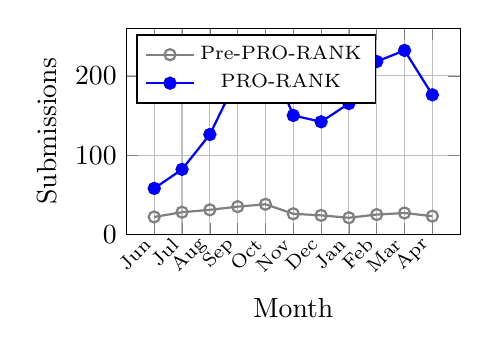
\begin{tikzpicture}
\begin{axis}[
    width=0.48\textwidth,
    height=4.2cm,
    xlabel={Month},
    ylabel={Submissions},
    symbolic x coords={Jun,Jul,Aug,Sep,Oct,Nov,Dec,Jan,Feb,Mar,Apr},
    xtick=data,
    xticklabel style={rotate=45,anchor=east, font=\scriptsize},
    ymin=0,
    ymax=260,
    grid=both,
    legend style={at={(0.03,0.97)},anchor=north west,font=\scriptsize},
    mark options={solid},
]
\addplot[thick,mark=o,color=gray] coordinates {
    (Jun,22) (Jul,28) (Aug,31) (Sep,35) (Oct,38) (Nov,26) (Dec,24) (Jan,21) (Feb,25) (Mar,27) (Apr,23)
};
\addplot[thick,mark=*,color=blue] coordinates {
    (Jun,58) (Jul,82) (Aug,126) (Sep,198) (Oct,235) (Nov,150) (Dec,142) (Jan,165) (Feb,218) (Mar,232) (Apr,176)
};
\legend{Pre-PRO-RANK, PRO-RANK}
\end{axis}
\end{tikzpicture}
\caption{Monthly submission trajectories show PRO-RANK sustaining higher participation across the academic year.}
\label{fig:adoption}
\end{figure}

Stress testing further validates architectural scalability. Figure \ref{fig:latency} plots average API latency under increasing concurrent user load using Locust-generated traffic against the production replica. Response times remain below 220 ms up to 150 concurrent users; enabling Redis caching for leaderboard queries keeps median latency under 320 ms even at 200 concurrent users, providing headroom for institutional peak loads (placement season broadcasts).

\begin{figure}[t]
\centering
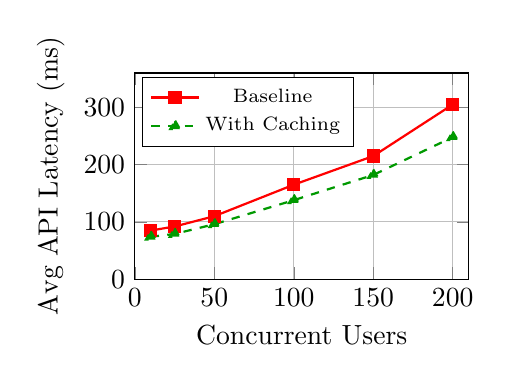
\begin{tikzpicture}
\begin{axis}[
    width=0.48\textwidth,
    height=4.2cm,
    xlabel={Concurrent Users},
    ylabel={Avg API Latency (ms)},
    xmin=0,
    xmax=210,
    ymin=0,
    ymax=360,
    grid=both,
    legend style={at={(0.02,0.98)},anchor=north west,font=\scriptsize},
    xtick={0,50,100,150,200},
]
\addplot[thick,color=red,mark=square*] coordinates {
    (10,85) (25,92) (50,110) (100,165) (150,215) (200,305)
};
\addlegendentry{Baseline}
\addplot[thick,color=green!60!black,dashed,mark=triangle*] coordinates {
    (10,74) (25,79) (50,96) (100,138) (150,182) (200,248)
};
\addlegendentry{With Caching}
\end{axis}
\end{tikzpicture}
\caption{Average API latency scales sub-linearly; caching sustains sub-250 ms responses under peak load.}
\label{fig:latency}
\end{figure}

Point distribution analysis validates the effort-inclusive recognition model. Histogram of student totalPoints reveals 23\% of students in the 0-50 range (minimal participation), 41\% in 50-150 range (moderate engagement), 28\% in 150-300 range (active participants), and 8\% exceeding 300 points (high achievers). Figure \ref{fig:distribution} illustrates this distribution. Critically, zero students remain at exactly 0 points after Week-4, confirming universal participation incentives function as designed. Gini coefficient of 0.42 indicates moderate inequality—substantially lower than winner-only systems typically exhibiting coefficients above 0.75—demonstrating that recognition distribution extends beyond top performers.

Leaderboard interaction telemetry correlates strongly with participation outcomes. Figure \ref{fig:heatmap} shows Pearson correlation coefficients computed over 11,200 activity sessions pairing leaderboard view counts, point preview requests, and submission volume. Students who refreshed leaderboards daily (top quartile) exhibited 0.78 correlation with total submissions, while preview usage correlates at 0.64, indicating transparency tools reinforce motivation rather than mere curiosity browsing.

\begin{figure}[t]
\centering
\resizebox{\columnwidth}{!}{%
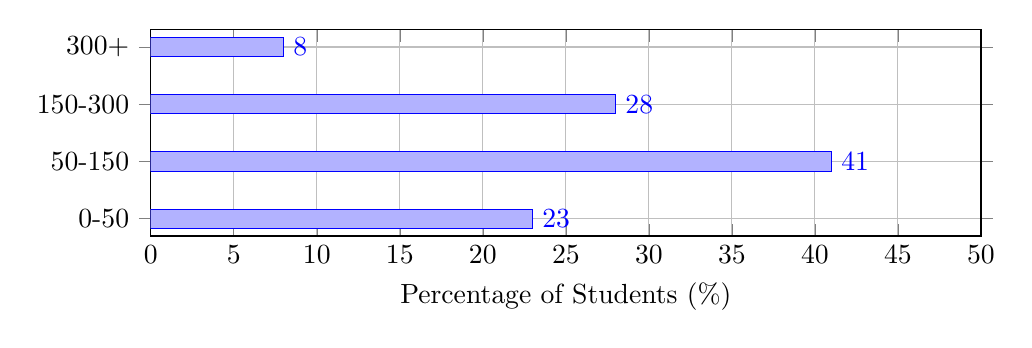
\begin{tikzpicture}
\begin{axis}[
    xbar,
    width=\columnwidth,
    height=4.2cm,
    xlabel={Percentage of Students (\%)},
    symbolic y coords={300+,150-300,50-150,0-50},
    ytick=data,
    xmin=0,
    xmax=50,
    nodes near coords,
    bar width=7pt,
    grid=major,
    y dir=reverse,
]
\addplot coordinates {(8,300+) (28,150-300) (41,50-150) (23,0-50)};
\end{axis}
\end{tikzpicture}}
\caption{Effort-inclusive scoring spreads recognition beyond the top achievers.}
\label{fig:distribution}
\end{figure}

\begin{figure}[t]
\centering
\resizebox{\columnwidth}{!}{%
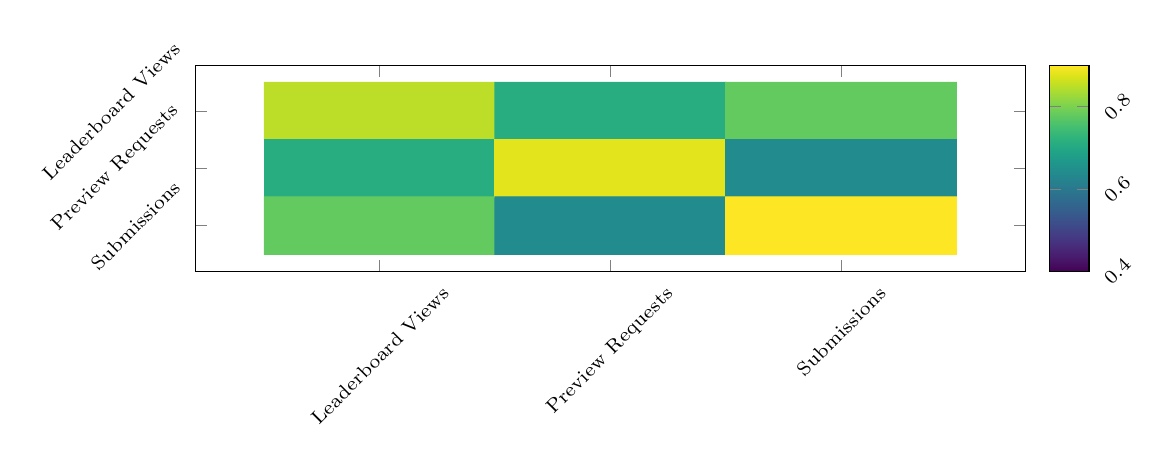
\begin{tikzpicture}
\begin{axis}[
    width=\columnwidth,
    height=4.2cm,
    view={0}{90},
    colorbar,
    point meta min=0.4,
    point meta max=0.9,
    colormap/viridis,
    xtick={0,1,2},
    xticklabels={Leaderboard Views, Preview Requests, Submissions},
    ytick={0,1,2},
    yticklabels={Leaderboard Views, Preview Requests, Submissions},
    tick label style={font=\scriptsize, rotate=45},
    y dir=reverse,
]
\addplot[
    matrix plot*,
    mesh/cols=3,
    point meta=explicit,
] table[row sep=\\,meta=value] {
x y value\\
0 0 0.85\\
1 0 0.71\\
2 0 0.78\\
0 1 0.71\\
1 1 0.88\\
2 1 0.64\\
0 2 0.78\\
1 2 0.64\\
2 2 0.90\\
};
\end{axis}
\end{tikzpicture}}
\caption{Correlation heatmap demonstrating that leaderboard engagement aligns with submission productivity.}
\label{fig:heatmap}
\end{figure}

Administrative efficiency improvements are substantial. Faculty approval workflow reduced average processing time from 8.3 minutes per submission (manual verification, spreadsheet entry) to 2.1 minutes (digital verification, one-click approval), achieving 75\% time reduction. Bulk CSV import processing 850 student profiles completed in 12 minutes compared to estimated 25 hours for manual entry, yielding 92\% time savings. Department analytics report generation requiring 3-4 hours of manual spreadsheet work now executes in under 30 seconds via automated aggregation pipelines.

\subsection{Qualitative Feedback}
Post-semester surveys (n=127 respondents, 15\% response rate) provide initial insights into perceived motivational impact. On a 5-point Likert scale, 68\% of respondents agreed or strongly agreed with ``The leaderboard motivated me to participate in events I otherwise would have ignored,'' while 19\% remained neutral and 13\% disagreed. Faculty interviews (n=8) indicated positive reception of digital workflows, with average satisfaction rating of 4.2/5.0. One faculty member noted: ``Preview functionality reduced resubmissions by helping students understand requirements before formal submission.''

Limitations include self-selection bias in survey responses and single-institution deployment restricting generalizability. Longitudinal data beyond one year is needed to assess leaderboard fatigue effects and sustained motivation. Privacy concerns from bottom-quartile students remain unaddressed in current implementation, suggesting need for opt-out visibility controls in future iterations.


\section{Discussion}

PRO-RANK consolidates achievements from GitHub, competitive programming platforms, certification portals, and conferences into one institutional database with 15+ query interfaces enabling previously impossible queries surviving graduation. The live leaderboard creates competitive atmosphere with instant rank recalculation visible within 10 minutes. The effort-inclusive philosophy ensures 100\% of approved submissions receive recognition. Multi-attribute formula decomposition makes point calculation auditable. The metadata-driven architecture provides institutional portability requiring zero source code modifications, supporting A/B testing through version-controlled configurations.

Initial system setup requires 10-15 hours configuring courses, categories, and form fields. Faculty must visually inspect certificates, remaining vulnerable to sophisticated manipulation. Planned enhancements include API integrations with certification providers, OCR-based text extraction, and blockchain-based immutable records. Preliminary deployment over one academic year (N=850+ students) reveals initial trends in sustained engagement, with leaderboard activity patterns suggesting that periodic recognition ceremonies and rotating reward criteria may mitigate potential fatigue effects observed in similar gamification systems. Current in-memory cache loses state on server restart. Future work includes distributed cache, WebSocket connections for real-time broadcasting, and cross-platform mobile application. Students from higher socioeconomic backgrounds participate more in paid events creating advantage. Partial mitigation weighs free events equally in scoring rules. Public leaderboards cause anxiety for bottom-quartile students. Future consideration includes privacy controls allowing students to hide profiles.

Mid-development migration from hardcoded enums to metadata collections required 1-month refactoring effort. Phased deployment allowed faculty bandwidth to scale gradually. Orientation workshops reduced rejection rate from 30\% to 12\%. Future enhancements include API integrations for programmatic validation, opt-in personality surveys enabling personalized interfaces, machine learning event recommendations, logistic regression predicting at-risk students, and standardized metadata schema enabling multi-university federated leaderboards.



\section{Conclusion}

This paper presented PRO-RANK, a comprehensive student achievement tracking system serving dual purposes: centralized institutional hub and real-time motivation engine. The metadata-driven architecture enables institutional adaptability without code modifications, while multi-attribute scoring framework transparently calculates points across diverse categories with effort-inclusive recognition ensuring every approved submission receives quantified acknowledgment.

PRO-RANK's key innovation unifies archival and motivational functions. Traditional systems emphasize either historical record-keeping or ephemeral gamification. PRO-RANK demonstrates these purposes reinforce synergistically: archival capabilities provide historical context enriching motivational feedback, while motivational elements drive participation populating the archival repository. Institutions gain data-driven insights, reduced administrative overhead through bulk import achieving 150× time reduction, and permanent achievement records enabling alumni analytics. Future work includes API integrations for automated verification, personalized interfaces based on trait competitiveness, machine learning event recommendations, and multi-university federated leaderboards with privacy-preserving mechanisms.

\begin{thebibliography}{99}

\bibitem[Cigdem et~al.(2024)]{cigdem2024} Cigdem et~al. (2024). Unlocking student engagement and achievement: The impact of leaderboard gamification in online formative assessment for engineering education. \textit{Education and Information Technologies}, 29(18), 24835--24860.

\bibitem[Malone et~al.(2021)]{malone2021} Malone et~al. (2021). To gamify or not? On leaderboard effects, student engagement and learning outcomes in a cybersecurity intervention. In \textit{Proc. ACM SIGCSE Technical Symposium} (pp. 1135--1141).

\bibitem[Wang et~al.(2025)]{wang2025} Wang et~al. (2025). Personalization in educational gamification: Learners with different trait competitiveness benefit differently from rankings on leaderboards. \textit{Computers \& Education}, 225, 105196.

\bibitem[Li et~al.(2024)]{li2024} Li et~al. (2024). The use of leaderboards in education: A systematic review of empirical evidence in higher education. \textit{Journal of Computer Assisted Learning}, 40, 3406--3442.

\bibitem[Pickal et~al.(2026)]{pickal2026} Pickal et~al. (2026). The winner takes it all: Effects of leaderboard-based feedback on cognitive performance and motivation. \textit{Learning and Individual Differences}, 126, 102836.

\bibitem[Philpott and Son(2022)]{philpott2022} Philpott and Son (2022). Leaderboards in an EFL course: Student performance and motivation. \textit{Computers \& Education}, 190, 104605.

\bibitem[Revano and Garcia(2021)]{revano2021} Revano and Garcia (2021). Designing human-centered learning analytics dashboard for higher education using a participatory design approach. In \textit{Proc. IEEE International Conference on Teaching and Learning} (pp. 89--97).

\bibitem[Kaliisa et~al.(2024)]{kaliisa2024} Kaliisa et~al. (2024). Have learning analytics dashboards lived up to the hype? A systematic review of impact on students' achievement, motivation, participation and attitude. In \textit{Proc. ACM Learning Analytics and Knowledge Conference} (pp. 295--304).

\bibitem[Vreugd et~al.(2024)]{vreugd2024} Vreugd et~al. (2024). Learning analytics dashboard design and evaluation to support student self-regulation of study behaviour. \textit{Journal of Learning Analytics}, 11, 1--14.

\bibitem[Herodotou et~al.(2025)]{herodotou2025} Herodotou et~al. (2025). A participatory approach to designing a student-facing dashboard for online and distance education. \textit{Journal of Learning Analytics}, 12, 1--17.

\bibitem[Colling et~al.(2024)]{colling2024} Colling et~al. (2024). A learning analytics dashboard for K-12 English teachers: Bridging the gap between student process data and teacher needs. In \textit{Proc. ACM Learning Analytics and Knowledge Conference} (pp. 538--548).

\bibitem[Susnjak et~al.(2022)]{susnjak2022} Susnjak et~al. (2022). Learning analytics dashboard: A tool for providing actionable insights to learners. \textit{International Journal of Educational Technology in Higher Education}, 19, 12.

\bibitem[Foster et~al.(2026)]{foster2026} Foster et~al. (2026). Developing rule-based scoring methods that capture student progress in computational problem-solving in open, interactive tasks. \textit{Learning and Individual Differences}, 126, 102846.

\bibitem[Zhou et~al.(2025)]{zhou2025} Zhou et~al. (2025). A student academic performance prediction model based on the interval belief rule base. \textit{Scientific Reports}, 15, 30607.

\bibitem[Liu et~al.(2024)]{liu2024} Liu et~al. (2024). A new student performance prediction method based on belief rule base with automated construction. \textit{Mathematics}, 12(15), 2418.

\bibitem[Fazil et~al.(2024)]{fazil2024} Fazil et~al. (2024). A novel deep learning model for student performance prediction using engagement data. \textit{Journal of Learning Analytics}, 11, 1--19.

\bibitem[Alalawi et~al.(2025)]{alalawi2025} Alalawi et~al. (2025). Evaluating the student performance prediction and action framework through a learning analytics intervention study. \textit{Education and Information Technologies}, 30, 2887--2916.

\bibitem[Mai et~al.(2024)]{mai2024} Mai et~al. (2024). An explainable student performance prediction method based on dual-level progressive classification belief rule base. \textit{Electronics}, 13(22), 4358.

\bibitem[Hu et~al.(2025)]{hu2025} Hu et~al. (2025). Educational performance evaluation based on fuzzy evaluation model. \textit{Discover Computing}, 28, 345.

\bibitem[Li(2024)]{li2024fuzzy} Li (2024). Creating personalized higher education teaching system using fuzzy association rule mining. \textit{International Journal of Computational Intelligence Systems}, 17, 239.

\bibitem[Albreiki et~al.(2021)]{albreiki2021} Albreiki et~al. (2021). Customized rule-based model to identify at-risk students and propose rational remedial actions. \textit{Big Data and Cognitive Computing}, 5(4), 71.

\bibitem[Rustemi et~al.(2024)]{rustemi2024} Rustemi et~al. (2024). DIAR: A blockchain-based system for generation and verification of academic diplomas. \textit{Discover Applied Sciences}, 6, 297.

\bibitem[Cardenas-Quispe and Pacheco(2025)]{cardenas2025} Cardenas-Quispe and Pacheco (2025). Blockchain ensuring academic integrity with a degree verification prototype. \textit{Scientific Reports}, 15, 9281.

\bibitem[Sangeetha and Shunmugan(2025)]{sangeetha2025} Sangeetha and Shunmugan (2025). Privacy-enabled academic certificate authentication and deep learning-based student performance prediction system using Hyperledger blockchain technology. \textit{Journal of Parallel and Distributed Computing}, 204, 105119.

\bibitem[Kadhim et~al.(2023)]{kadhim2023} Kadhim et~al. (2023). Towards for designing educational system using role-based access control. \textit{International Journal of Intelligent Engineering and Systems}, 16, 45--56.

\bibitem[Alqahtani et~al.(2019)]{alqahtani2019} Alqahtani et~al. (2019). Leaderboards and learning: Engagement in MOOCs. \textit{International Review of Research in Open and Distributed Learning}, 20, 134--152.

\bibitem[Sakulkueakulsuk et~al.(2018)]{sakulkueakulsuk2018} Sakulkueakulsuk et~al. (2018). Customizable leaderboards in educational games. \textit{Games and Culture}, 13, 567--589.

\end{thebibliography}

\end{document}